

\input{"C:/Users/spileggi/Google Drive/STAT 330/Lectures/SlideStyle.tex"}



\title[Lecture 1]{Introduction to SAS}
\author[Pileggi]{Shannon Pileggi}

\institute[STAT 330]{STAT 330}

\date{}


\begin{document}

\begin{frame}
\titlepage
\end{frame}

\begin{frame}
\frametitle{OUTLINE\qquad\qquad\qquad} \tableofcontents[hideallsubsections]
\end{frame}


%===========================================================================================================================
\section[Course overview]{Course overview}
%===========================================================================================================================

\subsection{}

\begin{frame}
\frametitle{About me}
Degrees
\begin{itemize}
\item BS Mathematics and Hispanic Studies
\item MS Biostatistics
\item PhD Biostatistics
\item[]
\end{itemize}

Personal
\begin{itemize}
\item Married, have a 2 year old daughter and 2 dogs
\item Enjoy: bike commuting, soccer, disc golf, hiking, board games
\item[]
\end{itemize}
\end{frame}

\begin{frame}
\frametitle{SAS versus R}
\bi
\item The two dominating statistical software packages are SAS and R
	\bi
	\item R is freeware (pros and cons)
	\item SAS is not free (pros and cons)
	\ei
\item SAS is superior at performing certain tasks compared to R
\item R is superior at performing certain tasks compared to SAS
\ei
\end{frame}

\begin{frame}
\frametitle{About SAS}
\bi
\item SAS (\ttb{S}tatistical \ttb{A}nalysis \ttb{S}ystem) was developed in the 1970s by a couple graduate students at NC State University.
\item The software is now simply known as `SAS' since its application extends beyond statistical analyses.
\item \textbf{THE WORLDWIDE LEADER} in industry as the main statistical toolbox software.
\item SAS consistently lands near the top of Fortune's annual list of best places to work.
\item \url{statweb.calpoly.edu/jdoi/web/classes/stat330/articleSAS.pdf}
\item \url{statweb.calpoly.edu/jdoi/web/classes/stat330/articleSAS2.pdf}
\ei
\end{frame}



%\begin{frame}
%\frametitle{What Can You Do with SAS?}
%\bi
%\item Import all sorts of data into SAS (a very powerful feature)
%\item Manipulate/clean data
%\item Simulate data
%\item Summarize data
%\item Perform statistical analyses
%\item Generate reports
%\ei
%\end{frame}

\begin{frame}
\frametitle{About this course}
\bi
\item This course will be more like a computer science class, where you learn the basics of a computing language
\item There is not a lot of statistical theory in this course, but the examples we use may build upon your previous statistics courses
\item You will learn a \emph{few} statistical analysis methods using SAS (e.g. t tests), but will focus \emph{more} on programming in SAS
\ei
\end{frame}


\begin{frame}
\frametitle{Learning objectives}
\begin{enumerate}
\item Formulate a game plan that states the objective before coding.
\item Identify multiple ways to achieve the game plan; consider pros and cons of the options before coding.
\item Apply techniques to prepare data for analysis, including: merging or transposing data, creating new variables, and identifying data errors and ``cleaning'' data.
\item Prepare summary statistics of data; create graphical displays of data.
\item Execute various statistical analyses and interpret results.
\item Apply arrays, loops, and SAS macros for efficient coding.
\item Discuss how SAS's progam data vector operates.
\item Import data of various sources and formats into SAS.
\item Verify that code renders the desired result in the presence of missing data.
\item[]
\end{enumerate}
\end{frame}




\begin{frame}
\frametitle{Course resources}
\bi
%\item Textbook: \tte{The Little SAS Book: A Primer}
%\item[]  Companion web site: \url{support.sas.com/companionsites}
%\item[]

\item Online Documentation \url{support.sas.com/documentation}
\item[]

\item SAS Proceedings \url{http://lexjansen.com/}
\item[]

\item Other helpful online resources from SAS Support
	\bi
	\item[] Knowledge Base \url{support.sas.com/resources}
	\item[] Support \url{support.sas.com/techsup}
	\item[] Training and Bookstore \url{support.sas.com/learn}
	\item[] Community \url{support.sas.com/community}
	\ei
\ei
\end{frame}

\begin{frame}
\frametitle{Acknowledgements}
A special thanks to the following institutions and instructors who have allowed me to borrow course notes and examples:
\bi
\item Rebecca Ottesen
\item Hunter Glanz
\item Jimmy Doi
\item SAS
\ei
\end{frame}

\begin{frame}
\frametitle{Other}
\bi
\item Review PolyLearn site
\item Discuss syllabus
\item Discuss ways to access SAS
\item Demonstrate shared directory
\ei
\end{frame}


%===========================================================================================================================
\section[Introduction to SAS]{Intro to SAS}
%===========================================================================================================================
\begin{frame}
\tableofcontents[currentsection, hideallsubsections]
\end{frame}
\subsection{}

\begin{frame}[fragile]
\fto
\bmp{0.7\textwidth}
\footnotesize
\begin{code}{.0}
/* Input data */
DATA grades;
   INPUT name $ exam1 exam2 exam3;
   DATALINES;
   Shannon      96    82    83
   Lex          92    81    68
   Becky        92    75    73
   ;
RUN;


/* Print data */
PROC PRINT DATA = grades;
RUN;
\end{code}
\emp
\end{frame}

\begin{frame}
\frametitle{SAS session: structure of windows}
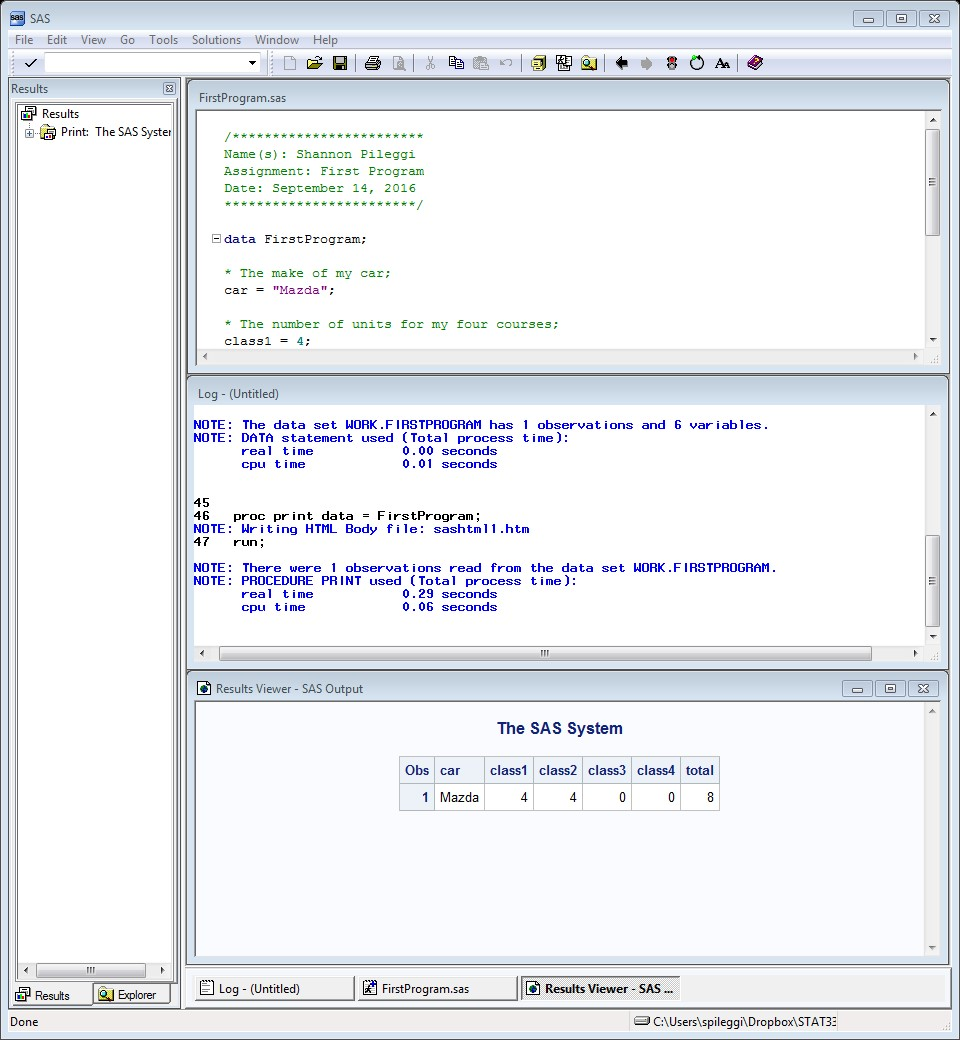
\includegraphics[width=0.7\textwidth]{FirstProgram.jpg}
\end{frame}

\begin{frame}
\ft{Windows}
\begin{enumerate}
\item \ttb{\ttu{Editor}}: SAS code is created here. Files saved from this window will have the \ttb{\ttt{.sas}} extension. Instead of using the regular ``Program Editor'', use the Enhanced Editor window (more user friendly).
\item \ttb{\ttu{Log}}: Messages pertaining to the successful (or unsuccessful) implementation of your code is listed here. Files saved from this window will have the \ttb{\ttt{.log}} extension.
\item  \ttb{\ttu{Results Viewer}}: If your code led to any text output, it will be stored here. Files saved from this window will have the \ttb{\ttt{.html}} extension.
\item \ttb{\ttu{Explorer}}: Access libraries and SAS data sets
\item[]
\end{enumerate}
\ttb{NOTE: If you want to save/print the contents of a particular window, be sure that it is `active' by using the mouse to click on it.}
\end{frame}

\begin{frame}
\ft{SAS programs}
SAS programs have two parts:
\begin{enumerate}
    \item Data steps: read and modify data
    \item Procedure (aka proc) steps: analyze data and produce reports
\end{enumerate}
\vskip10pt
\begin{clicker}{Our SAS program had \underline{\hspace{0.5in}} data step and \underline{\hspace{0.5in}} proc step.}
\begin{enumerate}
    \item 2; 0
    \item 0; 2
    \item 1; 1
    \item 1; 2
\end{enumerate}
\end{clicker}
\end{frame}


\begin{frame}
\ft{SAS data sets}
\bi
\item SAS works with its own data sets - raw data sets must be a SAS dat set or converted to a SAS data set before you can work with it.
\item Extensions for raw data sets can be almost anything - \ttb{\ttt{.dat}}, \ttb{\ttt{.txt}}, \ttb{\ttt{.xls}}, \ttb{\ttt{.csv}}, etc.
\item Extensions for SAS data sets:   \ttb{\ttt{.sas7bdat}}
\item SAS can handle many observations (rows) and variables (columns), which depends on your computer's memory.  (Prior to Version 9.1 SAS could accommodate 32,767 variables.)
\item SAS data sets are self-documenting - they contain information about when it was created, the number of observations and variables, variable types, etc.

\ei
\end{frame}


\begin{frame}
\frametitle{Data sets}
\begin{columns}
\column{0.25\textwidth}
\emph{Rows} indicate  \\
\textbf{observations} $\rightarrow$\\
\column{0.75\textwidth}
\hspace{0.5in} \textit{Columns} indicate \textbf{variables} \\
\hspace{1.3in}$\downarrow$ \\
\vskip10pt
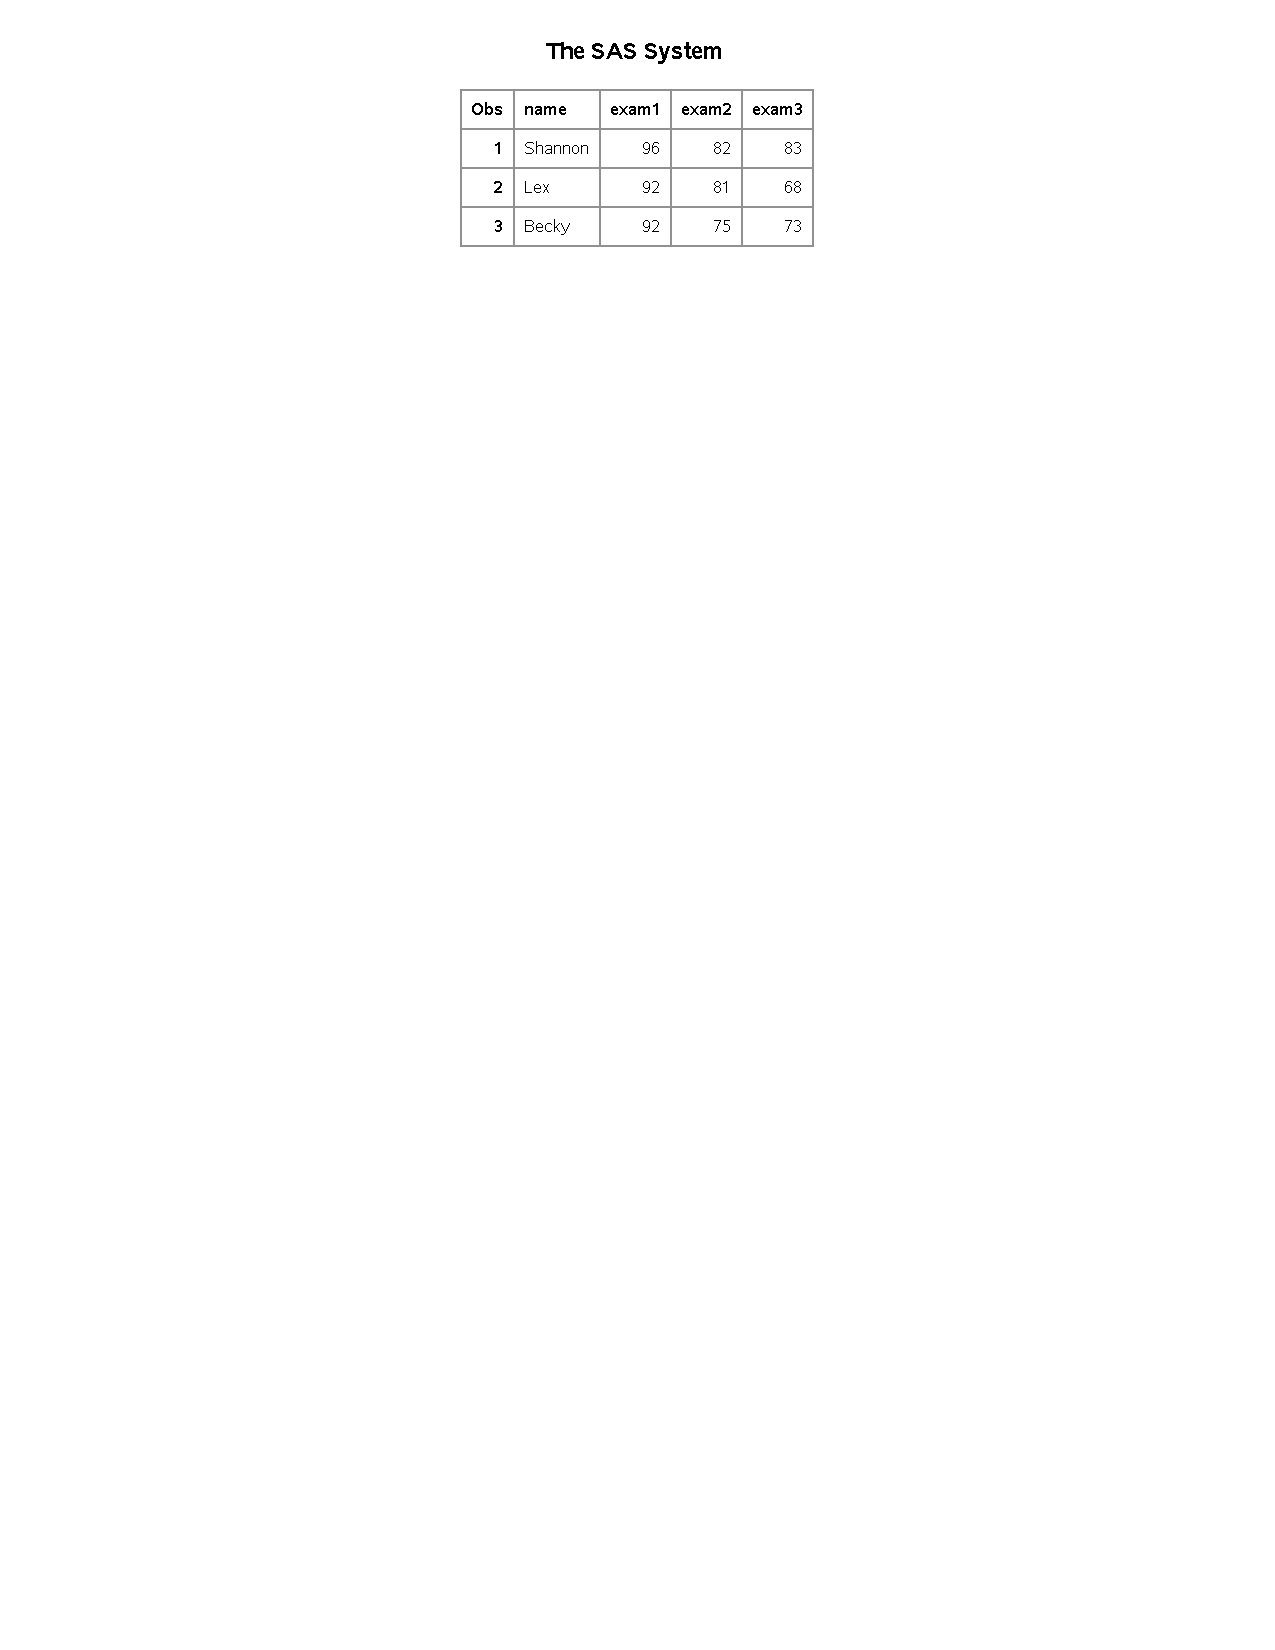
\includegraphics[trim={7cm 23cm 6cm 1.3cm},clip,width=1.0\textwidth]{L1_procprint.pdf}
\end{columns}
\vskip10pt
SAS data sets consist of two data types:
\begin{enumerate}
    \item \ttb{\ttu{Numeric}}: any numeral including +/-, dates (e.g. 01/03/2005),, decimal and scientific notation
    \item \ttb{\ttu{Character}}: Letters, numbers, special characters (up to 32,767, even in SAS v9.2)
\end{enumerate}
\end{frame}

\begin{frame}
\ft{Data types}
\bi
 \item If a variable contains letters or special characters, its data type is \tte{character}.
 \item If a variable contains all numbers, its data type can be either \tte{numeric} or \tte{character}.
 \item When deciding how to analyze your data, you should base your decision on what it represents in reality (eg, categorical versus quantitative).
\ei
\end{frame}

\begin{frame}
\begin{clicker}{Zip codes in the United States are 5 digit numbers (Cal Poly's is 93407).  If I had a data set with a variable for zip code of counties the SAS data type would likely be \underline{\hspace{1in}}, and in reality this would represent a \underline{\hspace{1in}} variable.}
\begin{enumerate}
    \item character; categorical
    \item character; quantitative
    \item numeric; categorical
    \item numeric; quantitative
\end{enumerate}
\end{clicker}
\end{frame}


\begin{frame}
\ft{Variable and data set names}
\bi
\item Must be 32 characters in length or less
\item Must start with a letter or underscore `\ttt{\myuscore}'
\item Can only contain letters, numbers, or underscores
\item Variable names are not case sensitive (the following variable names are equivalent: `Gender', `GENder', `GENDER', ...).
\item However, the values stored for a particular variable \textbf{are} case sensitive!
\ei
\end{frame}

\begin{frame}
\begin{clicker}{Which of the following are \underline{not} valid variable names?}
\begin{enumerate}
    \item \ttt{\myuscore}age
    \item Age.1
    \item 1age
    \item Age1
    \item ThisIsTheAgeWeStudy
    \item Age\ttt{\myuscore}1
    \item AgE
\end{enumerate}
\end{clicker}
\end{frame}

\begin{frame}
\ft{Missing data}
Many raw data sets contain missing observations. These are `stored' in SAS data sets according to the data type.
\bi
\item \small{If the missing data type is numeric, it is stored as a period: \ttb{\{.\}}}
\item \small{If the missing data type is character, it is stored as a blank: \ttb{\{\ \}}}
\ei
\vskip10pt
\begin{tabular}{rrrrr}
    \hline
    Name & Age & Gender & Height & Weight \\
    \hline\hline
    Max   & 33 & male   & .  & 204 \\
    Sally & 21 & female & 68 & 143 \\
    Susan & 25 &        & 65 & 142 \\
    Bob   & .  & male   & 73 & 215 \\
    \hline
\end{tabular}
\end{frame}

\begin{frame}
\ft{Comments in SAS code}
\bi
\item Following general programming etiquette, it is \textbf{ESSENTIAL} that you include comments in your SAS code!
\item This helps in making your code easier to read and reminds you why you may have coded things in a particular way.
\item Comments can be invoked in two ways:\\
    \qquad \qquad \ttb{\ttt{/* Anything placed here is a comment */}}\\
    \qquad \qquad \ttb{\ttt{* Anything placed here is a comment ;}}
\item Comments can span across multiple lines of code.
\item To quickly comment/uncomment a section of code:
	\bi
	\item Select the code section by highlighting with the cursor and then use \keys{Ctrl} + \keys{/}\\
	\item To uncomment any selected code simply use \keys{Ctrl} + \keys{Shift} + \keys{/}\\
	\ei
\ei
\end{frame}

\begin{frame}
\ft{Common errors}
\begin{itemize}
     \item Misspelling a variable name or SAS key word
    \item Forgetting a semi-colon
    \item \textbf{Every SAS statement ends with a semi-colon!}
    \item Always check your log
\end{itemize}
\vskip10pt
\oyo
Try removing a semi-colon or misspelling words to see what happens in your log.
\end{frame}

\begin{frame}
\ft{Debugging your code}
If you have an error in your code...
\bi
\item It is VERY VERY helpful to use the \ttt{/* ... */} style of comments to \emph{hide} sections of code
\item Move the comment marker to sequentially reveal code \textbf{one portion at a time}
\item By using this stepwise unveiling of code you should eventually be able to identify the error source(s)
\ei
\end{frame}

\begin{frame}[fragile]
\fto
Copy this code into the SAS editor and identify the 3 errors.
\bmp{0.7\textwidth}
\footnotesize
\begin{code}{.0}
DAT grades;
   INPUT name $ exam1 exam2 exam3;
   DATALINES;
   Shannon      96    82    83
   Lex          92    81    68
   Becky        92    75    73
   ;
RUN

PROC PRINT DATA = grade;
RUN;

\end{code}
\emp
\end{frame}

\begin{frame}
\ft{Saving your SAS code:}
\bi
\item It is good practice to \textbf{regularly} save SAS code (even if it's still a work in progress)
\item Be sure to have the Enhanced Editor window `active', then save your file.
\item Eventually, transfer all files to a personal storage device (flash drive, cloud storage, email, CD-Rom). The hard drives on the lab computers are wiped clean every evening!
\ei
\end{frame}



\begin{frame}
\frametitle{Shortcut Keys}
\bi
\item Go to Tools $\rightarrow$ Options $\rightarrow$ Keys (or \keys{F9})
\item[] Useful default keys:
\bi
\item \keys{F5} = \ttt{wpgm} = Enhanced Editor
\item \keys{F6} = \ttt{log} = Log Window
\item \keys{F7} = \ttt{output} = Output Window
\item \keys{F8} = \ttt{sub} = Submit SAS Code
\ei
\item Create your own key in \keys{F12} - do this every time you come to class!  This will greatly assist in identifying errors.
\item[] \ttb{\ttt{odsresults;clear;log;clear;wpgm;submit;log;top;}}
\ei
\end{frame}

\end{document} 